\title{2016 年高考数学 全国I卷-理科}
\date{}
\maketitle

\section*{一、单项选择题}
本大题共12小题，每小题5分，在每小题给出的四个选项中，只有一项是符合题目要求的.

\begin{question}[points=5]
设集合$A=\{x|x^2-4x+3<0\}$，$B=\{x|2x-3>0\}$，则$A\cap B=$（ ）
\begin{choices}
  \item $(-3,-\frac{3}{2})$
  \item $(-3,\frac{3}{2})$
  \item $(1,\frac{3}{2})$
  \item $(\frac{3}{2},3)$
\end{choices}
\begin{solution}
\textbf{答案：}D

\textbf{分析：}解不等式求出集合$A$，$B$，结合交集的定义，可得答案．

\textbf{详解：}解：∵集合$A=\{x|x^2-4x+3<0\}=(1,3)$，$B=\{x|2x-3>0\}=(\frac{3}{2},+\infty)$，∴$A\cap B=(\frac{3}{2},3)$，故选：D．
\end{solution}
\end{question}

\begin{question}[points=5]
设$(1+i)x=1+yi$，其中$x$，$y$是实数，则$|x+yi|=$（ ）
\begin{choices}
  \item $1$
  \item $\sqrt{2}$
  \item $\sqrt{3}$
  \item $2$
\end{choices}
\begin{solution}
\textbf{答案：}B

\textbf{分析：}根据复数相等求出$x$，$y$的值，结合复数的模长公式进行计算即可．

\textbf{详解：}解：∵$(1+i)x=1+yi$，∴$x+xi=1+yi$，即$\begin{cases}x=1\\x=y\end{cases}$，解得$\begin{cases}x=1\\y=1\end{cases}$，即$|x+yi|=|1+i|=\sqrt{2}$，故选：B．
\end{solution}
\end{question}

\begin{question}[points=5]
已知等差数列$\{a_n\}$前9项的和为27，$a_{10}=8$，则$a_{100}=$（ ）
\begin{choices}
  \item $100$
  \item $99$
  \item $98$
  \item $97$
\end{choices}
\begin{solution}
\textbf{答案：}C

\textbf{分析：}根据已知可得$a_5=3$，进而求出公差，可得答案．

\textbf{详解：}解：∵等差数列$\{a_n\}$前9项的和为27，$S_9=\frac{9(a_1+a_9)}{2}=9a_5$．∴$9a_5=27$，$a_5=3$，又∵$a_{10}=8$，∴$d=1$，∴$a_{100}=a_5+95d=98$，故选：C．
\end{solution}
\end{question}

\begin{question}[points=5]
某公司的班车在7:00，8:00，8:30发车，小明在7:50至8:30之间到达发车站乘坐班车，且到达发车站的时刻是随机的，则他等车时间不超过10分钟的概率是（ ）
\begin{choices}
  \item $\frac{1}{3}$
  \item $\frac{1}{2}$
  \item $\frac{2}{3}$
  \item $\frac{3}{4}$
\end{choices}
\begin{solution}
\textbf{答案：}B

\textbf{分析：}求出小明等车时间不超过10分钟的时间长度，代入几何概型概率计算公式，可得答案．

\textbf{详解：}解：设小明到达时间为$y$，当$y$在7:50至8:00，或8:20至8:30时，小明等车时间不超过10分钟，故$P=\frac{40}{40}=\frac{1}{2}$，故选：B．
\end{solution}
\end{question}

\begin{question}[points=5]
已知方程$\frac{x^2}{m^2+n}-\frac{y^2}{3m^2-n}=1$表示双曲线，且该双曲线两焦点间的距离为4，则$n$的取值范围是（ ）
\begin{choices}
  \item $(-1,3)$
  \item $(-1,\sqrt{3})$
  \item $(0,3)$
  \item $(0,\sqrt{3})$
\end{choices}
\begin{solution}
\textbf{答案：}A

\textbf{分析：}由已知可得$c=2$，利用$4=(m^2+n)+(3m^2-n)$，解得$m^2=1$，又$(m^2+n)(3m^2-n)>0$，从而可求$n$的取值范围．

\textbf{详解：}解：∵双曲线两焦点间的距离为4，∴$c=2$，当焦点在$x$轴上时，可得：$4=(m^2+n)+(3m^2-n)$，解得：$m^2=1$，∵方程$\frac{x^2}{m^2+n}-\frac{y^2}{3m^2-n}=1$表示双曲线，∴$(m^2+n)(3m^2-n)>0$，可得：$(n+1)(3-n)>0$，解得：$-1<n<3$，即$n$的取值范围是：$(-1,3)$．当焦点在$y$轴上时，无解．故选：A．
\end{solution}
\end{question}

\begin{question}[points=5]
如图，某几何体的三视图是三个半径相等的圆及每个圆中两条相互垂直的半径．若该几何体的体积是$\frac{28\pi}{3}$，则它的表面积是（ ）

\begin{center}
  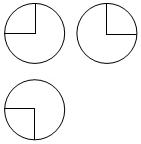
\includegraphics[width=.38\linewidth]{question-6-1.jpg}
\end{center}
\begin{choices}
  \item $17\pi$
  \item $18\pi$
  \item $20\pi$
  \item $28\pi$
\end{choices}
\begin{solution}
\textbf{答案：}A

\textbf{分析：}判断三视图复原的几何体的形状，利用体积求出几何体的半径，然后求解几何体的表面积．

\textbf{详解：}解：由题意可知三视图复原的几何体是一个球去掉$\frac{1}{8}$后的几何体，如图：可得：$\frac{7}{8}\times\frac{4}{3}\pi R^3=\frac{28\pi}{3}$，$R=2$．它的表面积是：$\frac{7}{8}\times4\pi\cdot2^2+\frac{3}{4}\pi\cdot2^2=17\pi$．故选：A．
\end{solution}
\end{question}

\begin{question}[points=5]
函数$y=2x^2-e^{|x|}$在$[-2,2]$的图象大致为（ ）

\begin{center}
  
\includegraphics[width=.38\linewidth]{question-7-1.jpg}
\end{center}
\begin{choices}
  \item A图像
  \item B图像
  \item C图像
  \item D图像
\end{choices}
\begin{solution}
\textbf{答案：}D

\textbf{分析：}根据已知中函数的解析式，分析函数的奇偶性，最大值及单调性，利用排除法，可得答案．

\textbf{详解：}解：∵$f(x)=y=2x^2-e^{|x|}$，∴$f(-x)=2(-x)^2-e^{|-x|}=2x^2-e^{|x|}$，故函数为偶函数，当$x=\pm2$时，$y=8-e^2\in(0,1)$，故排除$A$，$B$；当$x\in[0,2]$时，$f(x)=y=2x^2-e^x$，∴$f'(x)=4x-e^x=0$有解，故函数$y=2x^2-e^{|x|}$在$[0,2]$不是单调的，故排除$C$，故选：$D$．
\end{solution}
\end{question}

\begin{question}[points=5]
若$a>b>1$，$0<c<1$，则（ ）
\begin{choices}
  \item $a^c<b^c$
  \item $ab^c<ba^c$
  \item $a\log_b c<b\log_a c$
  \item $\log_a c<\log_b c$
\end{choices}
\begin{solution}
\textbf{答案：}C

\textbf{分析：}根据已知中$a>b>1$，$0<c<1$，结合对数函数和幂函数的单调性，分析各个结论的真假，可得答案．

\textbf{详解：}解：∵$a>b>1$，$0<c<1$，∴函数$f(x)=x^c$在$(0,+\infty)$上为增函数，故$a^c>b^c$，故$A$错误；函数$f(x)=x^{c-1}$在$(0,+\infty)$上为减函数，故$a^{c-1}<b^{c-1}$，故$ba^c<ab^c$，即$ab^c>ba^c$；故$B$错误；$\log_a c<0$，且$\log_b c<0$，$\log_a b<1$，即$\frac{\log_a c}{\log_b c}=\log_a b<1$，即$\log_a c>\log_b c$．故$D$错误；$0<-\log_a c<-\log_b c$，故$-b\log_a c<-a\log_b c$，即$b\log_a c>a\log_b c$，即$a\log_b c<b\log_a c$，故$C$正确；故选：$C$．
\end{solution}
\end{question}

\begin{question}[points=5]
执行下面的程序框图，如果输入的$x=0$，$y=1$，$n=1$，则输出$x$，$y$的值满足（ ）

\begin{center}
  
\includegraphics[width=.38\linewidth]{question-9-1.jpg}
\end{center}
\begin{choices}
  \item $y=2x$
  \item $y=3x$
  \item $y=4x$
  \item $y=5x$
\end{choices}
\begin{solution}
\textbf{答案：}C

\textbf{分析：}由已知中的程序框图可知：该程序的功能是利用循环结构计算并输出变量$x$，$y$的值，模拟程序的运行过程，分析循环中各变量值的变化情况，可得答案．

\textbf{详解：}解：输入$x=0$，$y=1$，$n=1$，则$x=0$，$y=1$，不满足$x^2+y^2\ge36$，故$n=2$，则$x=\frac{1}{2}$，$y=2$，不满足$x^2+y^2\ge36$，故$n=3$，则$x=\frac{3}{2}$，$y=6$，满足$x^2+y^2\ge36$，故$y=4x$，故选：$C$．
\end{solution}
\end{question}

\begin{question}[points=5]
以抛物线$C$的顶点为圆心的圆交$C$于$A$、$B$两点，交$C$的准线于$D$、$E$两点．已知$|AB|=4\sqrt{2}$，$|DE|=2\sqrt{5}$，则$C$的焦点到准线的距离为（ ）

\begin{center}
  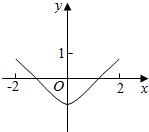
\includegraphics[width=.38\linewidth]{question-10-1.jpg}
\end{center}
\begin{choices}
  \item $2$
  \item $4$
  \item $6$
  \item $8$
\end{choices}
\begin{solution}
\textbf{答案：}B

\textbf{分析：}画出图形，设出抛物线方程，利用勾股定理以及圆的半径列出方程求解即可．

\textbf{详解：}解：设抛物线为$y^2=2px$，如图：$|AB|=4\sqrt{2}$，$|AM|=2\sqrt{2}$，$|DE|=2\sqrt{5}$，$|DN|=\sqrt{5}$，$|ON|=\frac{p}{2}$，$x_A=\frac{|AM|^2}{2p}=\frac{4}{p}$，$|OD|=|OA|$，$\left(\frac{p}{2}\right)^2+5=\frac{16}{p^2}+8$，解得：$p=4$．$C$的焦点到准线的距离为：$4$．故选：$B$．
\end{solution}
\end{question}

\begin{question}[points=5]
平面$\alpha$过正方体$ABCD-A_1B_1C_1D_1$的顶点$A$，$\alpha\parallel$平面$CB_1D_1$，$\alpha\cap$平面$ABCD=m$，$\alpha\cap$平面$ABB_1A_1=n$，则$m$、$n$所成角的正弦值为（ ）
\begin{choices}
  \item $\frac{\sqrt{3}}{2}$
  \item $\frac{\sqrt{2}}{2}$
  \item $\frac{\sqrt{3}}{3}$
  \item $\frac{1}{3}$
\end{choices}
\begin{solution}
\textbf{答案：}A

\textbf{分析：}画出图形，判断出$m$、$n$所成角，求解即可．

\textbf{详解：}解：如图：$\alpha\parallel$平面$CB_1D_1$，$\alpha\cap$平面$ABCD=m$，$\alpha\cap$平面$ABA_1B_1=n$，可知：$n\parallel CD_1$，$m\parallel B_1D_1$，∵$\triangle CB_1D_1$是正三角形．$m$、$n$所成角就是$\angle CD_1B_1=60^\circ$．则$m$、$n$所成角的正弦值为：$\frac{\sqrt{3}}{2}$．故选：$A$．
\end{solution}
\end{question}

\begin{question}[points=5]
已知函数$f(x)=\sin(\omega x+\varphi)$（$\omega>0$，$|\varphi|\le\frac{\pi}{2}$），$x=-\frac{\pi}{4}$为$f(x)$的零点，$x=\frac{\pi}{4}$为$y=f(x)$图象的对称轴，且$f(x)$在$(\frac{\pi}{18},\frac{5\pi}{36})$上单调，则$\omega$的最大值为（ ）
\begin{choices}
  \item $11$
  \item $9$
  \item $7$
  \item $5$
\end{choices}
\begin{solution}
\textbf{答案：}B

\textbf{分析：}根据已知可得$\omega$为正奇数，且$\omega\le12$，结合$x=-\frac{\pi}{4}$为$f(x)$的零点，$x=\frac{\pi}{4}$为$y=f(x)$图象的对称轴，求出满足条件的解析式，并结合$f(x)$在$(\frac{\pi}{18},\frac{5\pi}{36})$上单调，可得$\omega$的最大值．

\textbf{详解：}解：∵$x=-\frac{\pi}{4}$为$f(x)$的零点，$x=\frac{\pi}{4}$为$y=f(x)$图象的对称轴，∴$\frac{\pi}{4}-(-\frac{\pi}{4})=\frac{\pi}{2}=\frac{T}{4}+\frac{kT}{2}$，即$\frac{\pi}{2}=\frac{2\pi}{\omega}(\frac{1}{4}+\frac{k}{2})$，$\omega=2n+1$，$n\in N$即$\omega$为正奇数，∵$f(x)$在$(\frac{\pi}{18},\frac{5\pi}{36})$上单调，则$\frac{5\pi}{36}-\frac{\pi}{18}=\frac{\pi}{12}\le\frac{T}{2}$，即$T=\frac{2\pi}{\omega}\ge\frac{\pi}{6}$，解得：$\omega\le12$，当$\omega=11$时，$-\frac{11\pi}{4}+\varphi=k\pi$，$k\in Z$，∵$|\varphi|\le\frac{\pi}{2}$，∴$\varphi=-\frac{\pi}{4}$，此时$f(x)$在$(\frac{\pi}{18},\frac{5\pi}{36})$不单调，不满足题意；当$\omega=9$时，$-\frac{9\pi}{4}+\varphi=k\pi$，$k\in Z$，∵$|\varphi|\le\frac{\pi}{2}$，∴$\varphi=\frac{\pi}{4}$，此时$f(x)$在$(\frac{\pi}{18},\frac{5\pi}{36})$单调，满足题意；故$\omega$的最大值为$9$，故选：$B$．
\end{solution}
\end{question}

\section*{二、填空题}
本大题共4小题，每小题5分，共20分.

\begin{question}[points=5]
设向量$\vec{a}=(m,1)$，$\vec{b}=(1,2)$，且$|\vec{a}+\vec{b}|^2=|\vec{a}|^2+|\vec{b}|^2$，则$m=$．
\fillin[{$-2$}]
\begin{solution}
\textbf{答案：}$-2$

\textbf{分析：}利用已知条件，通过数量积判断两个向量垂直，然后列出方程求解即可．

\textbf{详解：}解：$|\vec{a}+\vec{b}|^2=|\vec{a}|^2+|\vec{b}|^2$，可得$\vec{a}\cdot\vec{b}=0$．向量$\vec{a}=(m,1)$，$\vec{b}=(1,2)$，可得$m+2=0$，解得$m=-2$．故答案为：$-2$．
\end{solution}
\end{question}

\begin{question}[points=5]
$(2x+\sqrt{x})^5$的展开式中，$x^3$的系数是．（用数字填写答案）
\fillin[{$10$}]
\begin{solution}
\textbf{答案：}$10$

\textbf{分析：}利用二项展开式的通项公式求出第$r+1$项，令$x$的指数为$3$，求出$r$，即可求出展开式中$x^3$的系数．

\textbf{详解：}解：$(2x+\sqrt{x})^5$的展开式中，通项公式为：$T_{r+1}=C_5^r(2x)^{5-r}(\sqrt{x})^r=2^{5-r}C_5^r x^{5-\frac{r}{2}}$，令$5-\frac{r}{2}=3$，解得$r=4$，∴$x^3$的系数$2^{1}C_5^4=10$．故答案为：$10$．
\end{solution}
\end{question}

\begin{question}[points=5]
设等比数列$\{a_n\}$满足$a_1+a_3=10$，$a_2+a_4=5$，则$a_1a_2\cdots a_n$的最大值为．
\fillin[{$64$}]
\begin{solution}
\textbf{答案：}$64$

\textbf{分析：}求出数列的等比与首项，化简$a_1a_2\cdots a_n$，然后求解最值．

\textbf{详解：}解：等比数列$\{a_n\}$满足$a_1+a_3=10$，$a_2+a_4=5$，可得$q(a_1+a_3)=5$，解得$q=\frac{1}{2}$．$a_1+q^2a_1=10$，解得$a_1=8$．则$a_1a_2\cdots a_n=a_1^n q^{1+2+3+\cdots+(n-1)}=8^n \left(\frac{1}{2}\right)^{\frac{n(n-1)}{2}}=2^{3n-\frac{n(n-1)}{2}}=2^{\frac{-n^2+7n}{2}}$，当$n=3$或$4$时，表达式取得最大值：$2^{\frac{-9+21}{2}}=2^6=64$．故答案为：$64$．
\end{solution}
\end{question}

\begin{question}[points=5]
某高科技企业生产产品$A$和产品$B$需要甲、乙两种新型材料．生产一件产品$A$需要甲材料$1.5kg$，乙材料$1kg$，用$5$个工时；生产一件产品$B$需要甲材料$0.5kg$，乙材料$0.3kg$，用$3$个工时，生产一件产品$A$的利润为$2100$元，生产一件产品$B$的利润为$900$元．该企业现有甲材料$150kg$，乙材料$90kg$，则在不超过$600$个工时的条件下，生产产品$A$、产品$B$的利润之和的最大值为元．
\fillin[{$216000$}]
\begin{solution}
\textbf{答案：}$216000$

\textbf{分析：}设$A$、$B$两种产品分别是$x$件和$y$件，根据题干的等量关系建立不等式组以及目标函数，利用线性规划作出可行域，通过目标函数的几何意义，求出其最大值即可；

\textbf{详解：}解：设$A$、$B$两种产品分别是$x$件和$y$件，获利为$z$元．由题意，得$\begin{cases}1.5x+0.5y\le150\\x+0.3y\le90\\5x+3y\le600\\x\ge0,y\ge0\end{cases}$，$z=2100x+900y$．不等式组表示的可行域如图：由题意可得$\begin{cases}5x+3y=600\\x+0.3y=90\end{cases}$，解得：$\begin{cases}x=60\\y=100\end{cases}$，$A(60,100)$，目标函数$z=2100x+900y$．经过$A$时，直线的截距最大，目标函数取得最大值：$2100\times60+900\times100=216000$元．故答案为：$216000$．
\end{solution}
\end{question}

\section*{三、解答题}
本大题共5小题，满分60分，解答须写出文字说明、证明过程或演算步骤.

\begin{question}[points=12]
$\triangle ABC$的内角$A$，$B$，$C$的对边分别为$a$，$b$，$c$，已知$2\cos C(a\cos B+b\cos A)=c$．

（Ⅰ）求$C$；

（Ⅱ）若$c=\sqrt{7}$，$\triangle ABC$的面积为$\frac{3\sqrt{3}}{2}$，求$\triangle ABC$的周长．
\begin{solution}
\textbf{答案：}（Ⅰ）$C=\frac{\pi}{3}$；（Ⅱ）$5+\sqrt{7}$

\textbf{分析：}（Ⅰ）已知等式利用正弦定理化简，整理后利用两角和与差的正弦函数公式及诱导公式化简，根据$\sin C$不为$0$求出$\cos C$的值，即可确定出出$C$的度数；（2）利用余弦定理列出关系式，利用三角形面积公式列出关系式，求出$a+b$的值，即可求$\triangle ABC$的周长．

\textbf{详解：}解：（Ⅰ）∵在$\triangle ABC$中，$0<C<\pi$，∴$\sin C\neq0$已知等式利用正弦定理化简得：$2\cos C(\sin A\cos B+\sin B\cos A)=\sin C$，整理得：$2\cos C\sin(A+B)=\sin C$，即$2\cos C\sin(\pi-(A+B))=\sin C$，$2\cos C\sin C=\sin C$，∴$\cos C=\frac{1}{2}$，∴$C=\frac{\pi}{3}$；（Ⅱ）由余弦定理得$7=a^2+b^2-2ab\cdot\frac{1}{2}$，∴$(a+b)^2-3ab=7$，∵$S=\frac{1}{2}ab\sin C=\frac{\sqrt{3}}{4}ab=\frac{3\sqrt{3}}{2}$，∴$ab=6$，∴$(a+b)^2-18=7$，∴$a+b=5$，∴$\triangle ABC$的周长为$5+\sqrt{7}$．
\end{solution}
\end{question}

\begin{question}[points=12]
如图，在以$A$，$B$，$C$，$D$，$E$，$F$为顶点的五面体中，面$ABEF$为正方形，$AF=2FD$，$\angle AFD=90^\circ$，且二面角$D-AF-E$与二面角$C-BE-F$都是$60^\circ$．

（Ⅰ）证明平面$ABEF\perp$平面$EFDC$；

（Ⅱ）求二面角$E-BC-A$的余弦值．

\begin{center}
  
\includegraphics[width=.38\linewidth]{question-18-1.jpg}
\end{center}
\begin{solution}
\textbf{答案：}（Ⅰ）证明见解析；（Ⅱ）$-\frac{\sqrt{19}}{19}$

\textbf{分析：}（Ⅰ）证明$AF\perp$平面$EFDC$，利用平面与平面垂直的判定定理证明平面$ABEF\perp$平面$EFDC$；（Ⅱ）证明四边形$EFDC$为等腰梯形，以$E$为原点，建立如图所示的坐标系，求出平面$BEC$、平面$ABC$的法向量，代入向量夹角公式可得二面角$E-BC-A$的余弦值．

\textbf{详解：}（Ⅰ）证明：∵$ABEF$为正方形，∴$AF\perp EF$．∵$\angle AFD=90^\circ$，∴$AF\perp DF$，∵$DF\cap EF=F$，∴$AF\perp$平面$EFDC$，∵$AF\subset$平面$ABEF$，∴平面$ABEF\perp$平面$EFDC$；（Ⅱ）解：由$AF\perp DF$，$AF\perp EF$，可得$\angle DFE$为二面角$D-AF-E$的平面角；由$ABEF$为正方形，$AF\perp$平面$EFDC$，∵$BE\perp EF$，∴$BE\perp$平面$EFDC$即有$CE\perp BE$，可得$\angle CEF$为二面角$C-BE-F$的平面角．可得$\angle DFE=\angle CEF=60^\circ$．∵$AB\parallel EF$，$AB\not\subset$平面$EFDC$，$EF\subset$平面$EFDC$，∴$AB\parallel$平面$EFDC$，∵平面$EFDC\cap$平面$ABCD=CD$，$AB\subset$平面$ABCD$，∴$AB\parallel CD$，∴$CD\parallel EF$，∴四边形$EFDC$为等腰梯形．以$E$为原点，建立如图所示的坐标系，设$FD=a$，则$E(0,0,0)$，$B(0,2a,0)$，$C(\frac{a}{2},0,\frac{\sqrt{3}}{2}a)$，$A(2a,2a,0)$，∴$\overrightarrow{EB}=(0,2a,0)$，$\overrightarrow{BC}=(\frac{a}{2},-2a,\frac{\sqrt{3}}{2}a)$，$\overrightarrow{AB}=(-2a,0,0)$设平面$BEC$的法向量为$\vec{n}=(x_1,y_1,z_1)$，则$\begin{cases}\vec{n}\cdot\overrightarrow{EB}=0\\\vec{n}\cdot\overrightarrow{BC}=0\end{cases}$，即$\begin{cases}2ay_1=0\\\frac{a}{2}x_1-2ay_1+\frac{\sqrt{3}}{2}az_1=0\end{cases}$，取$\vec{n}=(\sqrt{3},0,-1)$．设平面$ABC$的法向量为$\vec{m}=(x_2,y_2,z_2)$，则$\begin{cases}\vec{m}\cdot\overrightarrow{AB}=0\\\vec{m}\cdot\overrightarrow{BC}=0\end{cases}$，即$\begin{cases}-2ax_2=0\\\frac{a}{2}x_2-2ay_2+\frac{\sqrt{3}}{2}az_2=0\end{cases}$，取$\vec{m}=(0,\sqrt{3},4)$．设二面角$E-BC-A$的大小为$\theta$，则$\cos\theta=\frac{\vec{n}\cdot\vec{m}}{|\vec{n}||\vec{m}|}=\frac{-4}{2\cdot\sqrt{19}}=-\frac{\sqrt{19}}{19}$，则二面角$E-BC-A$的余弦值为$-\frac{\sqrt{19}}{19}$．
\end{solution}
\end{question}

\begin{question}[points=12]
某公司计划购买$2$台机器，该种机器使用三年后即被淘汰．机器有一易损零件，在购进机器时，可以额外购买这种零件作为备件，每个$200$元．在机器使用期间，如果备件不足再购买，则每个$500$元．现需决策在购买机器时应同时购买几个易损零件，为此搜集并整理了$100$台这种机器在三年使用期内更换的易损零件数，得如图柱状图：以这$100$台机器更换的易损零件数的频率代替$1$台机器更换的易损零件数发生的概率，记$X$表示$2$台机器三年内共需更换的易损零件数，$n$表示购买$2$台机器的同时购买的易损零件数．

（Ⅰ）求$X$的分布列；

（Ⅱ）若要求$P(X\le n)\ge0.5$，确定$n$的最小值；

（Ⅲ）以购买易损零件所需费用的期望值为决策依据，在$n=19$与$n=20$之中选其一，应选用哪个？

\begin{center}
  
\includegraphics[width=.38\linewidth]{question-19-1.jpg}
\end{center}
\begin{solution}
\textbf{答案：}（Ⅰ）分布列见解析；（Ⅱ）$n$的最小值为$19$；（Ⅲ）应选$n=19$

\textbf{分析：}（Ⅰ）由已知得$X$的可能取值为$16$，$17$，$18$，$19$，$20$，$21$，$22$，分别求出相应的概率，由此能求出$X$的分布列．（Ⅱ）由$X$的分布列求出$P(X\le18)=\frac{3}{10}$，$P(X\le19)=\frac{7}{10}$．由此能确定满足$P(X\le n)\ge0.5$中$n$的最小值．（Ⅲ）法一：由$X$的分布列得$P(X\le19)=\frac{7}{10}$．求出买$19$个所需费用期望$EX_1$和买$20$个所需费用期望$EX_2$，由此能求出买$19$个更合适．法二：购买零件所用费用含两部分，一部分为购买零件的费用，另一部分为备件不足时额外购买的费用，分别求出$n=19$时，费用的期望和当$n=20$时，费用的期望，从而得到买$19$个更合适．

\textbf{详解：}解：（Ⅰ）由已知得$X$的可能取值为$16$，$17$，$18$，$19$，$20$，$21$，$22$，$P(X=16)=(\frac{20}{100})^2=\frac{1}{25}$，$P(X=17)=2\times\frac{20}{100}\times\frac{20}{100}=\frac{2}{25}$，$P(X=18)=(\frac{20}{100})^2+2\times(\frac{20}{100})^2=\frac{3}{25}$，$P(X=19)=2\times\frac{20}{100}\times\frac{40}{100}+2\times\frac{20}{100}\times\frac{20}{100}=\frac{12}{50}=\frac{6}{25}$，$P(X=20)=2\times\frac{20}{100}\times\frac{20}{100}+(\frac{40}{100})^2=\frac{8}{50}=\frac{4}{25}$，$P(X=21)=2\times\frac{40}{100}\times\frac{20}{100}=\frac{4}{25}$，$P(X=22)=(\frac{20}{100})^2=\frac{1}{25}$，∴$X$的分布列为：$\begin{array}{c|ccccccc} X & 16 & 17 & 18 & 19 & 20 & 21 & 22 \\ \hline P & \frac{1}{25} & \frac{2}{25} & \frac{3}{25} & \frac{6}{25} & \frac{4}{25} & \frac{4}{25} & \frac{1}{25} \end{array}$（Ⅱ）由（Ⅰ）知：$P(X\le18)=P(X=16)+P(X=17)+P(X=18)=\frac{1}{25}+\frac{2}{25}+\frac{3}{25}=\frac{6}{25}=\frac{3}{10}$．$P(X\le19)=P(X=16)+P(X=17)+P(X=18)+P(X=19)=\frac{1}{25}+\frac{2}{25}+\frac{3}{25}+\frac{6}{25}=\frac{12}{25}=\frac{7}{10}$．∴$P(X\le n)\ge0.5$中，$n$的最小值为$19$．（Ⅲ）解法一：由（Ⅰ）得$P(X\le19)=\frac{7}{10}$．买$19$个所需费用期望：$EX_1=200\times\frac{3}{10}+(200\times19+500)\times\frac{4}{25}+(200\times19+500\times2)\times\frac{4}{25}+(200\times19+500\times3)\times\frac{1}{25}=4040$，买$20$个所需费用期望：$EX_2=200\times\frac{7}{10}+(200\times20+500)\times\frac{4}{25}+(200\times20+2\times500)\times\frac{1}{25}=4080$，∵$EX_1<EX_2$，∴买$19$个更合适．解法二：购买零件所用费用含两部分，一部分为购买零件的费用，另一部分为备件不足时额外购买的费用，当$n=19$时，费用的期望为：$19\times200+500\times0.2+1000\times0.08+1500\times0.04=4040$，当$n=20$时，费用的期望为：$20\times200+500\times0.08+1000\times0.04=4080$，∴买$19$个更合适．
\end{solution}
\end{question}

\begin{question}[points=12]
设圆$x^2+y^2+2x-15=0$的圆心为$A$，直线$l$过点$B(1,0)$且与$x$轴不重合，$l$交圆$A$于$C$，$D$两点，过$B$作$AC$的平行线交$AD$于点$E$．

（Ⅰ）证明$|EA|+|EB|$为定值，并写出点$E$的轨迹方程；

（Ⅱ）设点$E$的轨迹为曲线$C_1$，直线$l$交$C_1$于$M$，$N$两点，过$B$且与$l$垂直的直线与圆$A$交于$P$，$Q$两点，求四边形$MPNQ$面积的取值范围．
\begin{solution}
\textbf{答案：}（Ⅰ）$|EA|+|EB|=4$，轨迹方程为$\frac{x^2}{4}+\frac{y^2}{3}=1$（$y\neq0$）；（Ⅱ）$[12,8\sqrt{3})$

\textbf{分析：}（Ⅰ）求得圆$A$的圆心和半径，运用直线平行的性质和等腰三角形的性质，可得$EB=ED$，再由圆的定义和椭圆的定义，可得$E$的轨迹为以$A$，$B$为焦点的椭圆，求得$a$，$b$，$c$，即可得到所求轨迹方程；（Ⅱ）设直线$l:x=my+1$，代入椭圆方程，运用韦达定理和弦长公式，可得$|MN|$，由$PQ\perp l$，设$PQ:y=-m(x-1)$，求得$A$到$PQ$的距离，再由圆的弦长公式可得$|PQ|$，再由四边形的面积公式，化简整理，运用不等式的性质，即可得到所求范围．

\textbf{详解：}解：（Ⅰ）证明：圆$x^2+y^2+2x-15=0$即为$(x+1)^2+y^2=16$，可得圆心$A(-1,0)$，半径$r=4$，由$BE\parallel AC$，可得$\angle C=\angle EBD$，由$AC=AD$，可得$\angle D=\angle C$，即为$\angle D=\angle EBD$，即有$EB=ED$，则$|EA|+|EB|=|EA|+|ED|=|AD|=4$，故$E$的轨迹为以$A$，$B$为焦点的椭圆，且有$2a=4$，即$a=2$，$c=1$，$b=\sqrt{a^2-c^2}=\sqrt{3}$，则点$E$的轨迹方程为$\frac{x^2}{4}+\frac{y^2}{3}=1$（$y\neq0$）；（Ⅱ）椭圆$C_1:\frac{x^2}{4}+\frac{y^2}{3}=1$，设直线$l:x=my+1$，由$PQ\perp l$，设$PQ:y=-m(x-1)$，由$\begin{cases}\frac{x^2}{4}+\frac{y^2}{3}=1\\x=my+1\end{cases}$可得$(3m^2+4)y^2+6my-9=0$，设$M(x_1,y_1)$，$N(x_2,y_2)$，可得$y_1+y_2=-\frac{6m}{3m^2+4}$，$y_1y_2=-\frac{9}{3m^2+4}$，则$|MN|=\sqrt{1+m^2}\cdot|y_1-y_2|=\sqrt{1+m^2}\cdot\sqrt{(y_1+y_2)^2-4y_1y_2}=\sqrt{1+m^2}\cdot\sqrt{\frac{36m^2}{(3m^2+4)^2}+\frac{36}{3m^2+4}}=12\cdot\frac{1+m^2}{3m^2+4}$，$A$到$PQ$的距离为$d=\frac{|0+m(-1-1)|}{\sqrt{1+m^2}}=\frac{|2m|}{\sqrt{1+m^2}}$，$|PQ|=2\sqrt{r^2-d^2}=2\sqrt{16-\frac{4m^2}{1+m^2}}=4\sqrt{\frac{3m^2+4}{1+m^2}}$，则四边形$MPNQ$面积为$S=\frac{1}{2}|PQ|\cdot|MN|=\frac{1}{2}\cdot4\sqrt{\frac{3m^2+4}{1+m^2}}\cdot12\cdot\frac{1+m^2}{3m^2+4}=24\sqrt{\frac{1+m^2}{3m^2+4}}=24\sqrt{\frac{1}{3+\frac{1}{1+m^2}}}$，当$m=0$时，$S$取得最小值$12$，又$\frac{1}{1+m^2}>0$，可得$S<24\sqrt{\frac{1}{3}}=8\sqrt{3}$，即有四边形$MPNQ$面积的取值范围是$[12,8\sqrt{3})$．
\end{solution}
\end{question}

\begin{question}[points=12]
已知函数$f(x)=(x-2)e^x+a(x-1)^2$有两个零点．

（Ⅰ）求$a$的取值范围；

（Ⅱ）设$x_1$，$x_2$是$f(x)$的两个零点，证明：$x_1+x_2<2$．
\begin{solution}
\textbf{答案：}（Ⅰ）$(0,+\infty)$；（Ⅱ）证明见解析

\textbf{分析：}（Ⅰ）由函数$f(x)=(x-2)e^x+a(x-1)^2$可得：$f'(x)=(x-1)e^x+2a(x-1)=(x-1)(e^x+2a)$，对$a$进行分类讨论，综合讨论结果，可得答案．（Ⅱ）设$x_1$，$x_2$是$f(x)$的两个零点，则$-a=\frac{(x_1-2)e^{x_1}}{(x_1-1)^2}=\frac{(x_2-2)e^{x_2}}{(x_2-1)^2}$，令$g(x)=\frac{(x-2)e^x}{(x-1)^2}$，则$g(x_1)=g(x_2)=-a$，分析$g(x)$的单调性，令$m>0$，则$g(1+m)-g(1-m)=\frac{(m-1)e^{1+m}}{m^2}-\frac{(-m-1)e^{1-m}}{m^2}=\frac{e[ (m-1)e^m - (-m-1)e^{-m}]}{m^2}$，设$h(m)= (m-1)e^m + (m+1)e^{-m}$，$m>0$，利用导数法可得$h(m)>h(0)=0$恒成立，即$g(1+m)>g(1-m)$恒成立，令$m=1-x_1>0$，可得结论．

\textbf{详解：}解：（Ⅰ）∵函数$f(x)=(x-2)e^x+a(x-1)^2$，∴$f'(x)=(x-1)e^x+2a(x-1)=(x-1)(e^x+2a)$，①若$a=0$，那么$f(x)=0\Leftrightarrow(x-2)e^x=0\Leftrightarrow x=2$，函数$f(x)$只有唯一的零点$2$，不合题意；②若$a>0$，那么$e^x+2a>0$恒成立，当$x<1$时，$f'(x)<0$，此时函数为减函数；当$x>1$时，$f'(x)>0$，此时函数为增函数；此时当$x=1$时，函数$f(x)$取极小值$-e$，由$f(2)=a>0$，可得：函数$f(x)$在$x>1$存在一个零点；当$x<1$时，$e^x<e$，$x-2<-1<0$，∴$f(x)=(x-2)e^x+a(x-1)^2>(x-2)e+a(x-1)^2=a(x-1)^2+e(x-1)-e$，令$a(x-1)^2+e(x-1)-e=0$的两根为$t_1$，$t_2$，且$t_1<t_2$，则当$x<t_1$，或$x>t_2$时，$f(x)>a(x-1)^2+e(x-1)-e>0$，故函数$f(x)$在$x<1$存在一个零点；即函数$f(x)$在$R$是存在两个零点，满足题意；③若$-\frac{e}{2}<a<0$，则$\ln(-2a)<\ln e=1$，当$x<\ln(-2a)$时，$x-1<\ln(-2a)-1<\ln e-1=0$，$e^x+2a<e^{\ln(-2a)}+2a=0$，即$f'(x)=(x-1)(e^x+2a)>0$恒成立，故$f(x)$单调递增，当$\ln(-2a)<x<1$时，$x-1<0$，$e^x+2a>e^{\ln(-2a)}+2a=0$，即$f'(x)=(x-1)(e^x+2a)<0$恒成立，故$f(x)$单调递减，当$x>1$时，$x-1>0$，$e^x+2a>e^{\ln(-2a)}+2a=0$，即$f'(x)=(x-1)(e^x+2a)>0$恒成立，故$f(x)$单调递增，故当$x=\ln(-2a)$时，函数取极大值，由$f(\ln(-2a))=[\ln(-2a)-2](-2a)+a[\ln(-2a)-1]^2=a\{[\ln(-2a)-2]^2+1\}<0$得：函数$f(x)$在$R$上至多存在一个零点，不合题意；④若$a=-\frac{e}{2}$，则$\ln(-2a)=1$，当$x<1=\ln(-2a)$时，$x-1<0$，$e^x+2a<e^{\ln(-2a)}+2a=0$，即$f'(x)=(x-1)(e^x+2a)>0$恒成立，故$f(x)$单调递增，当$x>1$时，$x-1>0$，$e^x+2a>e^{\ln(-2a)}+2a=0$，即$f'(x)=(x-1)(e^x+2a)>0$恒成立，故$f(x)$单调递增，故函数$f(x)$在$R$上单调递增，函数$f(x)$在$R$上至多存在一个零点，不合题意；⑤若$a<-\frac{e}{2}$，则$\ln(-2a)>\ln e=1$，当$x<1$时，$x-1<0$，$e^x+2a<e^{\ln(-2a)}+2a=0$，即$f'(x)=(x-1)(e^x+2a)>0$恒成立，故$f(x)$单调递增，当$1<x<\ln(-2a)$时，$x-1>0$，$e^x+2a<e^{\ln(-2a)}+2a=0$，即$f'(x)=(x-1)(e^x+2a)<0$恒成立，故$f(x)$单调递减，当$x>\ln(-2a)$时，$x-1>0$，$e^x+2a>e^{\ln(-2a)}+2a=0$，即$f'(x)=(x-1)(e^x+2a)>0$恒成立，故$f(x)$单调递增，故当$x=1$时，函数取极大值，由$f(1)=-e<0$得：函数$f(x)$在$R$上至多存在一个零点，不合题意；综上所述，$a$的取值范围为$(0,+\infty)$证明：（Ⅱ）∵$x_1$，$x_2$是$f(x)$的两个零点，∴$f(x_1)=f(x_2)=0$，且$x_1\neq1$，且$x_2\neq1$，∴$-a=\frac{(x_1-2)e^{x_1}}{(x_1-1)^2}=\frac{(x_2-2)e^{x_2}}{(x_2-1)^2}$，令$g(x)=\frac{(x-2)e^x}{(x-1)^2}$，则$g(x_1)=g(x_2)=-a$，∵$g'(x)=\frac{[(x-1)-1]e^x(x-1)-2(x-2)e^x}{(x-1)^3}=\frac{e^x[(x-1)^2- (x-1)-2(x-2)]}{(x-1)^3}=\frac{e^x[(x-1)^2-3x+5]}{(x-1)^3}$，当$x<1$时，$g'(x)<0$，$g(x)$单调递减；当$x>1$时，$g'(x)>0$，$g(x)$单调递增；设$m>0$，则$g(1+m)-g(1-m)=\frac{(m-1)e^{1+m}}{m^2}-\frac{(-m-1)e^{1-m}}{m^2}=\frac{e[(m-1)e^m+(m+1)e^{-m}]}{m^2}$，设$h(m)= (m-1)e^m+(m+1)e^{-m}$，$m>0$，则$h'(m)= e^m+(m-1)e^m + e^{-m}-(m+1)e^{-m}= me^m - me^{-m}= m(e^m - e^{-m})>0$恒成立，即$h(m)$在$(0,+\infty)$上为增函数，$h(m)>h(0)=0$恒成立，即$g(1+m)>g(1-m)$恒成立，令$m=1-x_1>0$，则$g(1+1-x_1)>g(1-1+x_1)\Leftrightarrow g(2-x_1)>g(x_1)=g(x_2)\Leftrightarrow 2-x_1>x_2$，即$x_1+x_2<2$．
\end{solution}
\end{question}

\section*{四、选考题（选修4-1：几何证明选讲）}
请考生在22、23、24题中任选一题作答，如果多做，则按所做的第一题计分.

\begin{question}[points=10]
如图，$\triangle OAB$是等腰三角形，$\angle AOB=120^\circ$．以$O$为圆心，$\frac{1}{2}OA$为半径作圆．

（Ⅰ）证明：直线$AB$与$\odot O$相切；

（Ⅱ）点$C$，$D$在$\odot O$上，且$A$，$B$，$C$，$D$四点共圆，证明：$AB\parallel CD$．
\begin{solution}
\textbf{答案：}（Ⅰ）证明见解析；（Ⅱ）证明见解析

\textbf{分析：}（Ⅰ）设$K$为$AB$中点，连结$OK$．根据等腰三角形$AOB$的性质知$OK\perp AB$，$\angle A=30^\circ$，$OK=OA\sin30^\circ=\frac{1}{2}OA$，则$AB$是圆$O$的切线．（Ⅱ）设圆心为$T$，证明$OT$为$AB$的中垂线，$OT$为$CD$的中垂线，即可证明结论．

\textbf{详解：}证明：（Ⅰ）设$K$为$AB$中点，连结$OK$，∵$OA=OB$，$\angle AOB=120^\circ$，∴$OK\perp AB$，$\angle A=30^\circ$，$OK=OA\sin30^\circ=\frac{1}{2}OA$，∴直线$AB$与$\odot O$相切；（Ⅱ）因为$OA=2OD$，所以$O$不是$A$，$B$，$C$，$D$四点所在圆的圆心．设$T$是$A$，$B$，$C$，$D$四点所在圆的圆心．∵$OA=OB$，$TA=TB$，∴$OT$为$AB$的中垂线，同理，$OC=OD$，$TC=TD$，∴$OT$为$CD$的中垂线，∴$AB\parallel CD$．
\end{solution}
\end{question}

\section*{五、选考题（选修4-4：坐标系与参数方程）}

\begin{question}[points=10]
在直角坐标系$xOy$中，曲线$C_1$的参数方程为$\begin{cases}x=a\cos t\\ y=1+a\sin t\end{cases}$（$t$为参数，$a>0$）．在以坐标原点为极点，$x$轴正半轴为极轴的极坐标系中，曲线$C_2:\rho=4\cos\theta$．

（Ⅰ）说明$C_1$是哪种曲线，并将$C_1$的方程化为极坐标方程；

（Ⅱ）直线$C_3$的极坐标方程为$\theta=\alpha_0$，其中$\alpha_0$满足$\tan\alpha_0=2$，若曲线$C_1$与$C_2$的公共点都在$C_3$上，求$a$．
\begin{solution}
\textbf{答案：}（Ⅰ）$C_1$为以$(0,1)$为圆心，$a$为半径的圆，极坐标方程为$\rho^2-2\rho\sin\theta+1-a^2=0$；（Ⅱ）$a=1$

\textbf{分析：}（Ⅰ）把曲线$C_1$的参数方程变形，然后两边平方作和即可得到普通方程，可知曲线$C_1$是圆，化为一般式，结合$x^2+y^2=\rho^2$，$y=\rho\sin\theta$化为极坐标方程；（Ⅱ）化曲线$C_2$、$C_3$的极坐标方程为直角坐标方程，由条件可知$y=2x$为圆$C_1$与$C_2$的公共弦所在直线方程，把$C_1$与$C_2$的方程作差，结合公共弦所在直线方程为$y=2x$可得$1-a^2=0$，则$a$值可求．

\textbf{详解：}解：（Ⅰ）由$\begin{cases}x=a\cos t\\ y=1+a\sin t\end{cases}$，得$\begin{cases}\frac{x}{a}=\cos t\\ \frac{y-1}{a}=\sin t\end{cases}$，两式平方相加得，$x^2+(y-1)^2=a^2$．∴$C_1$为以$(0,1)$为圆心，以$a$为半径的圆．化为一般式：$x^2+y^2-2y+1-a^2=0$．①由$x^2+y^2=\rho^2$，$y=\rho\sin\theta$，得$\rho^2-2\rho\sin\theta+1-a^2=0$；（Ⅱ）$C_2:\rho=4\cos\theta$，两边同时乘$\rho$得$\rho^2=4\rho\cos\theta$，∴$x^2+y^2=4x$，②即$(x-2)^2+y^2=4$．由$C_3:\theta=\alpha_0$，其中$\alpha_0$满足$\tan\alpha_0=2$，得$y=2x$，∵曲线$C_1$与$C_2$的公共点都在$C_3$上，∴$y=2x$为圆$C_1$与$C_2$的公共弦所在直线方程，①-②得：$4x-2y+1-a^2=0$，即为$C_3$，∴$1-a^2=0$，∴$a=1$（$a>0$）．
\end{solution}
\end{question}

\section*{六、选考题（选修4-5：不等式选讲）}

\begin{question}[points=10]
已知函数$f(x)=|x+1|-|2x-3|$．

（Ⅰ）在图中画出$y=f(x)$的图象；

（Ⅱ）求不等式$|f(x)|>1$的解集．

\begin{center}
  
\includegraphics[width=.38\linewidth]{question-24-1.jpg}
\end{center}
\begin{solution}
\textbf{答案：}（Ⅰ）图象见解析；（Ⅱ）$(-\infty,\frac{1}{3})\cup(1,3)\cup(5,+\infty)$

\textbf{分析：}（Ⅰ）运用分段函数的形式写出$f(x)$的解析式，由分段函数的画法，即可得到所求图象；（Ⅱ）分别讨论当$x\le-1$时，当$-1<x<\frac{3}{2}$时，当$x\ge\frac{3}{2}$时，解绝对值不等式，取交集，最后求并集即可得到所求解集．

\textbf{详解：}解：（Ⅰ）$f(x)=\begin{cases} x-4, & x\le-1 \\ 3x-2, & -1<x<\frac{3}{2} \\ 4-x, & x\ge\frac{3}{2} \end{cases}$，由分段函数的图象画法，可得$f(x)$的图象，如右：（Ⅱ）由$|f(x)|>1$，可得当$x\le-1$时，$|x-4|>1$，解得$x>5$或$x<3$，即有$x\le-1$；当$-1<x<\frac{3}{2}$时，$|3x-2|>1$，解得$x>1$或$x<\frac{1}{3}$，即有$-1<x<\frac{1}{3}$或$1<x<\frac{3}{2}$；当$x\ge\frac{3}{2}$时，$|4-x|>1$，解得$x>5$或$x<3$，即有$x>5$或$\frac{3}{2}\le x<3$．综上可得，$x<\frac{1}{3}$或$1<x<3$或$x>5$．则$|f(x)|>1$的解集为$(-\infty,\frac{1}{3})\cup(1,3)\cup(5,+\infty)$．
\end{solution}
\end{question}

